% !TEX root =./main.tex

\section{Block 4: Upsampling (2x)}

Upsampling involves increasing the number of samples by interpolating the existing data.  In this case, we are upsampling our data so that we are able to form more beams, and thus have a higher resolution image.

The goal for the upsampling block is to double the number of samples.  In order to do this, there are two steps.  First, zeros must be added in between the datapoints.  Second, the zero-padded data must be low pass filtered with 
\begin{align*}
    f_c = \frac{F_{s,old}}{2} = 50 \unit{kHz}
\end{align*}
to remove the reflected image of the data.

\subsection{Implementation}

We must implement both of these steps in a very fast way, without sacrificing quality.

First, \textsc{Matlab} is meant for working with vectorized functions, and has vectorized methods of replacing certain indexes.  Thus, the quickest way to add a zero after every sample (double the number of samples) is to replace every other entry of a matrix of zeros with the data point.

Second, in order to interpolate, we will use the minimum order filter possible that preserves the necessary information, because a lower order results in less multiplies and thus a quicker function.  Additionally, FIR was chosen in order to preserve the relative phase of the received signals, which is necessary for preventing distortion in the sonar image.  Equirriple was used as the design method.

In this case, an order 3 filter with the specifications in Table \ref{tab:upsample_filter} works.  Our information is contained in the band less than $20 \unit{kHz}$, and thus we can set $f_{pass}$ to $20 \unit{kHz}$.  Then, because our $F_{s,old} = 100 \unit{kHz}$, there is a significant amount of bandwidth between our data's frequency spectrum and its reflected image.  Thus, we can set $f_{stop}$ to be $69 \unit{kHz}$, the sharpest it can be while still being order 3.  Through various trials, an $A_{stop}$ of $40 \unit{dB}$ sufficiently suppresses the image, will also allowing the filter to be order 3.

\begin{table}[H]
    \centering
    \begin{tabular}{c|cccc}
        Order & Fpass & Fstop & Apass & Astop \\ \hline
        3 & $20  \unit{kHz}$ & $69  \unit{kHz}$ & $1  \unit{dB} $ & $40  \unit{dB}$
    \end{tabular}
    \caption{Parameters for Upsampling Low Pass Filter}
    \label{tab:upsample_filter}
\end{table}

The frequency response of the low pass filter can be seen in Figure \ref{fig:upsample_freq_response}.

\begin{figure}[H]
    \centering
    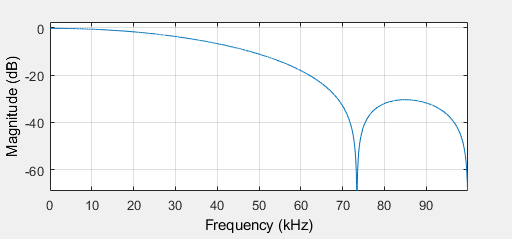
\includegraphics[width=0.5\linewidth]{figures/upsample_freq_response.png}
    \caption{Frequency Response of Upsampling Low Pass Filter}
    \label{fig:upsample_freq_response}
\end{figure}

In order to preserve this speed, the function header was modified to accept the numerator taps of the low pass filter, matrix of zeros, and the length of the matrix of zeros as input in addition to the data to be upsampled.


\subsection{Analysis}

An initial, simple test to confirm that the function upsamples properly is by inspecting a linear function.  This can be seen in Figure \ref{fig:linear_upsample_whole}. 

\begin{figure}[H]
    \centering
    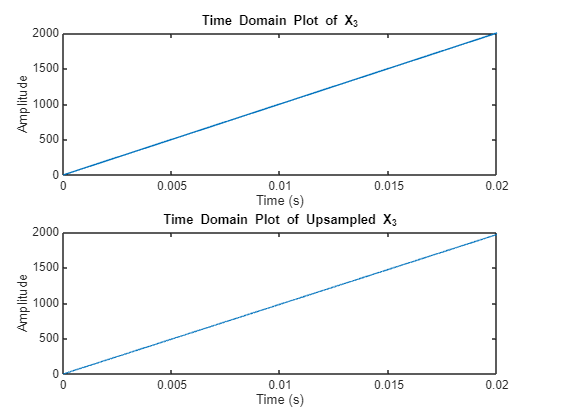
\includegraphics[width=0.5\linewidth]{figures/linear_upsample_whole.png}
    \caption{Upsampled Linear Function}
    \label{fig:linear_upsample_whole}
\end{figure}

It can be seen  in Figure \ref{fig:linear_upsample_zoom} that the upsampled version contains the same data, but has twice as many points.

\begin{figure}[H]
    \centering
    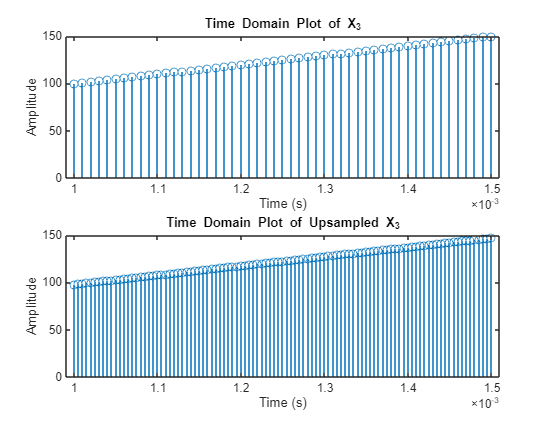
\includegraphics[width=0.5\linewidth]{figures/linear_upsample_zoom.png}
    \caption{Zoomed Portion of Upsampled Linear Function}
    \label{fig:linear_upsample_zoom}
\end{figure}

Testing on various other types of synthetic data, such as sinusoids and linear combinations of sinusoids, further confirmed that the function was implemented as intended.  

As the next test, we can upsample the provided test data (unmodified by the other stages) to ensure it has no unintended effects.  As can be seen in Figure \ref{fig:upsample_time} and Figure \ref{fig:upsample_freq}, te data was interoplated correctly.  Each channel is represented by a color.

\begin{figure}[H]
    \centering
    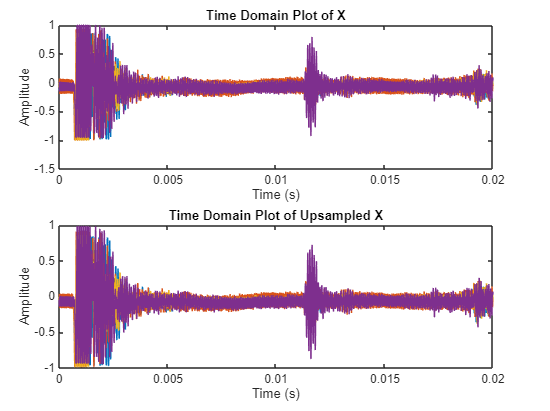
\includegraphics[width=0.5\linewidth]{figures/upsample_time.png}
    \caption{Upsampled Data in Time}
    \label{fig:upsample_time}
\end{figure}

\begin{figure}[H]
    \centering
    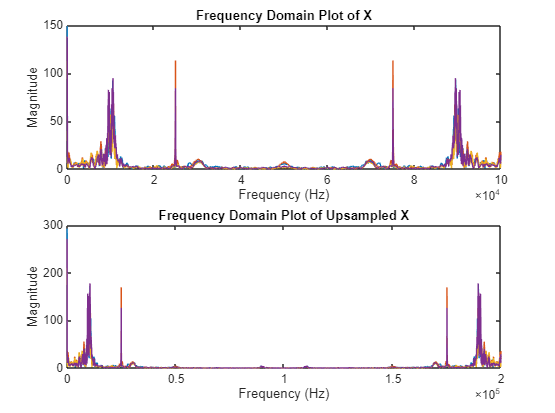
\includegraphics[width=0.5\linewidth]{figures/upsample_freq.png}
    \caption{Upsampled Data in Frequency}
    \label{fig:upsample_freq}
\end{figure}

Zooming in for Figure \ref{fig:upsample_time_zoom} and Figure \ref{fig:upsample_freq_zoom}, we can more clearly see that the interpolation was successful.

\begin{figure}[H]
    \centering
    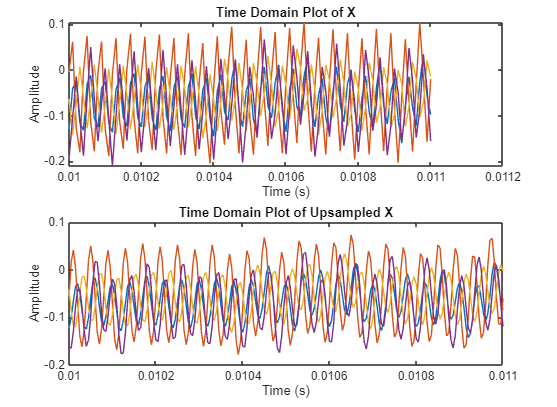
\includegraphics[width=0.5\linewidth]{figures/upsample_time_zoom.png}
    \caption{Zoomed Portion of Upsampled Data in Time}
    \label{fig:upsample_time_zoom}
\end{figure}

\begin{figure}[H]
    \centering
    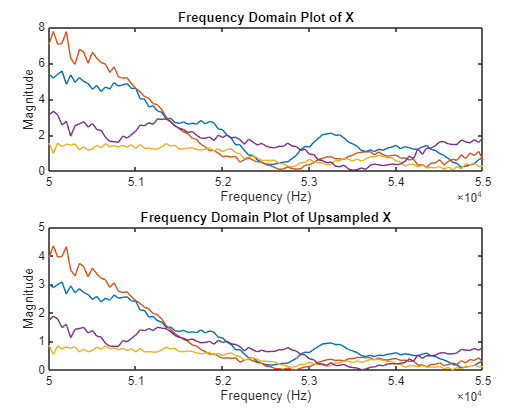
\includegraphics[width=0.5\linewidth]{figures/upsample_freq_zoom.png}
    \caption{Zoomed Portion of Upsampled Data in Frequency}
    \label{fig:upsample_freq_zoom}
\end{figure}

Therefore, the function successfully interpolates the data at a high quality.  The next step in the analysis is in the timing.  Benchmarking is difficult, but here we are only comparing the newly written function to the provided \code{.p} file.  In this case, each function was timed (using \code{tic} and \code{toc}) over $10,000$ iterations, and the average runtimes can be seen in Table \ref{tab:upsampleFunctionTime}.  The same data (the provided test data) was used, and the computer was in as similar a state as possible.

\begin{table}[H]
    \centering
    \begin{tabular}{cc}
        Function & Time ($\mu$s) \\ \hline
        Provided \code{.p} & $5455$\\
        Rewritten \code{.m} & $64.7$
    \end{tabular}
    \caption{Parameters for Upsampling Low Pass Filter}
    \label{tab:upsampleFunctionTime}
\end{table}

Therefore, the rewritten \code{upsampling.m} function provides a high quality upsampling by $2$ and is about 100 times faster than the original function.